\documentclass[11pt]{article}
\usepackage[a4paper, total={6.8in, 9.25in}]{geometry}
\usepackage{graphicx}
\graphicspath{ {./assets/images/output/} }
\usepackage{caption}
\usepackage[english]{babel}
\usepackage{float}
\usepackage{amsmath}
\usepackage{amssymb}
\usepackage{minted}
\usepackage{multicol}
\usepackage{array}
\usepackage{setspace}
\usepackage{placeins}
\usepackage{tcolorbox}
\usepackage{subcaption}

\definecolor{verbgray}{gray}{.95}
\setminted{
    bgcolor=verbgray,
    baselinestretch=1,
    fontsize=\footnotesize,
    linenos,
    breaklines=true,
    breakanywhere=true,
    xleftmargin=\parindent
}

\pagenumbering{gobble}
\begin{document}
\captionsetup{justification=centering}

% Custom cover page handles the title block
\input{dip_cover.tex}
\pagebreak

% Table of Contents will now properly nest subsections under each Experiment
\tableofcontents
\pagebreak
\pagenumbering{arabic}


% EXPERIMENT 5

\begin{center}
    \section{Experiment 5: Image Thresholding}
\end{center}

\subsection{Theory and Introduction}
Image thresholding is a fundamental method of image segmentation. It is used to convert a grayscale image into a binary image (black and white) by separating objects of interest from the background based on their pixel intensity \cite{gonzalez2018}. A threshold value $T$ is selected, and each pixel is evaluated against this value:
$$
    g(x,y) = \begin{cases}
        1, & \text{if } f(x,y) \ge T \\
        0, & \text{if } f(x,y) < T
    \end{cases}
$$
This experiment explores the manual implementation of this thresholding logic without relying on built-in binarization functions.

\subsection{Methodology}
A grayscale matrix was evaluated, and conditional logic was applied pixel-by-pixel to generate the binary output.

\subsubsection{Matrix Definition}
A $5 \times 5$ matrix with an increasing gradient of intensity values (ranging from 10 to 255) was defined to clearly observe the boundary created by the threshold.
$$
    I = \begin{bmatrix}
        10  & 50  & 100 & 150 & 200 \\
        30  & 80  & 120 & 180 & 220 \\
        60  & 110 & 140 & 210 & 250 \\
        90  & 130 & 170 & 230 & 240 \\
        120 & 160 & 190 & 245 & 255
    \end{bmatrix}
$$
A threshold value of $T = 127$ was selected.

\subsubsection{Python Implementation}
The implementation avoids built-in thresholding functions. An empty array of zeros was created, and nested loops were utilized to iterate through every coordinate. The intensity value was checked against $T$, and the corresponding output pixel was set to 1 (or 255 for visualization) or 0.

\begin{multicols}{2}
    \inputminted{python3}{./assets/lab5.py}
\end{multicols}

\subsection{Results}
The code generated a segmented binary matrix, visualized in the figure below.

\begin{figure}[H]
    \centering
    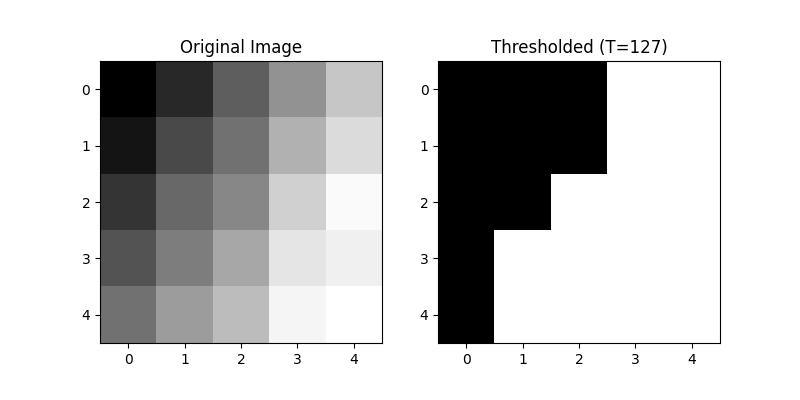
\includegraphics[width=0.8\linewidth]{lab5.png}
    \caption{Image Thresholding ($T=127$). Left: Original grayscale gradient. Right: The resulting binary image showing a clear step-edge segmentation.}
    \label{fig:threshold}
\end{figure}

\subsection{Discussion}
The manual conditional mapping successfully segmented the matrix. As observed in the results, all pixels with an intensity $\ge 127$ (located towards the bottom right) were assigned the foreground value (white), while those $< 127$ (top left) were assigned the background value (black). This created a clear diagonal boundary, demonstrating how thresholding groups similar intensity regions.

\subsection{Conclusion}
The underlying mathematical principle of binary segmentation was validated. By manually applying the threshold piecewise function via iterative loops, it was confirmed that object isolation can be achieved strictly through simple intensity condition checks.

\pagebreak
% EXPERIMENT 6
\begin{center}
    \section{Experiment 6: Linear Contrast Stretching}
\end{center}

\subsection{Theory and Introduction}
Linear contrast stretching is a spatial domain enhancement technique used to expand the dynamic range of an image \cite{gonzalez2018}. It employs a piecewise linear transformation function defined by critical points $(r_1, s_1)$ and $(r_2, s_2)$. The transformation is divided into three regions—dark, mid-tone, and bright—each governed by a distinct slope ($\alpha, \beta, \gamma$):
\begin{itemize}
    \item \textbf{Dark region ($0 \to r_1$):} Slope $\alpha = \frac{s_1}{r_1}$
    \item \textbf{Mid-tone region ($r_1 \to r_2$):} Slope $\beta = \frac{s_2 - s_1}{r_2 - r_1}$
    \item \textbf{Bright region ($r_2 \to L-1$):} Slope $\gamma = \frac{(L-1) - s_2}{(L-1) - r_2}$
\end{itemize}

\subsection{Methodology}
The piecewise slopes were calculated, and the transformation was mapped across the pixels of a standard test image (Lenna) to enhance contrast.

\subsubsection{Parameter Definition}
The input parameters were defined as $r_1 = 70, r_2 = 180$ and target values $s_1 = 40, s_2 = 220$. The maximum intensity level was set to $L-1 = 255$.

\subsubsection{Python Implementation}
The slopes $\alpha, \beta,$ and $\gamma$ were computed mathematically. Nested loops were used to evaluate each pixel and apply the corresponding linear equation based on which intensity region the pixel occupied.

\begin{multicols}{2}
    \inputminted{python3}{./assets/lab6.py}
\end{multicols}

\subsection{Results}
The transformation stretched the mid-tones while compressing extreme shadows and highlights.

\begin{figure}[H]
    \centering
    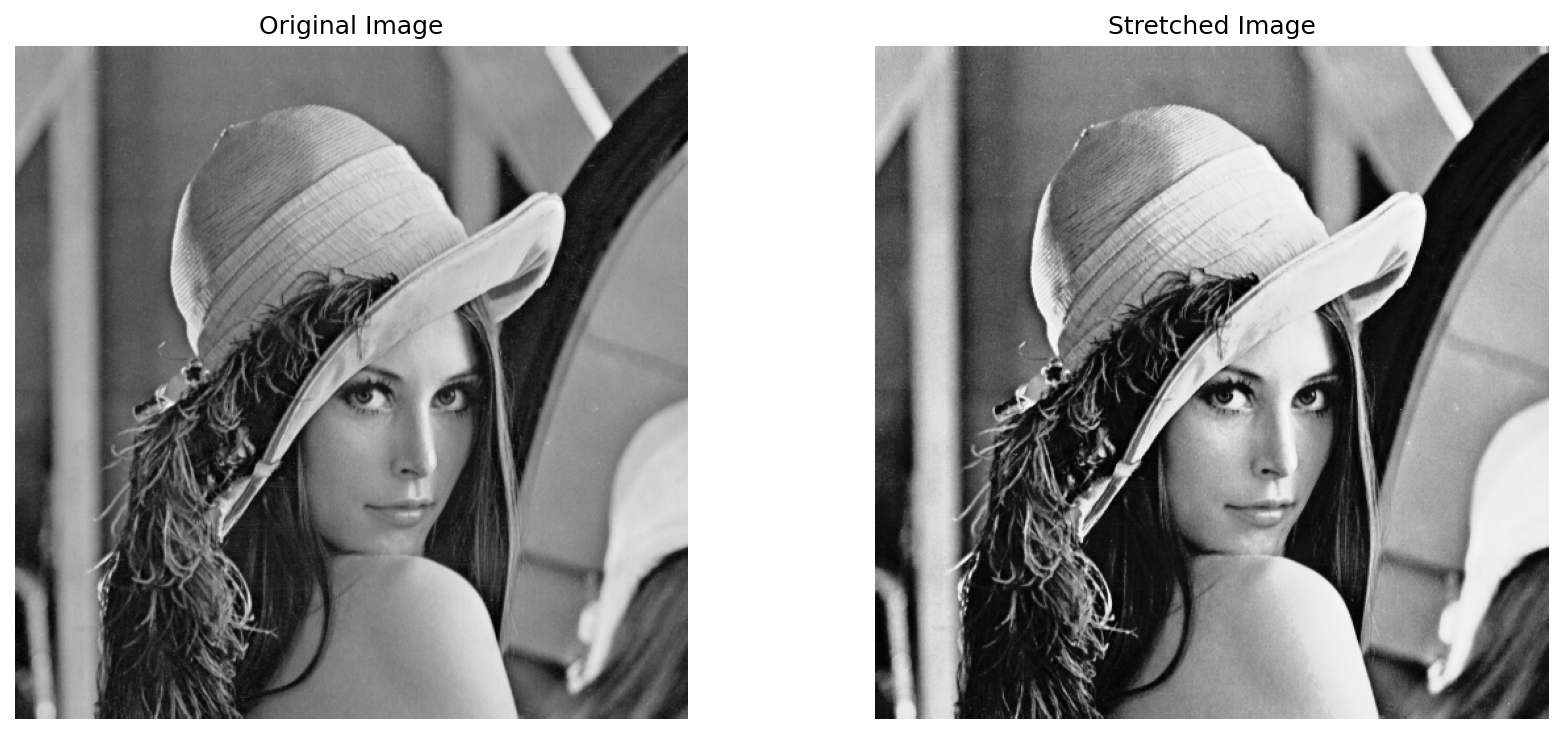
\includegraphics[width=\linewidth]{lab6.png}
    \caption{Contrast Stretching Results. Left: Original low-contrast image. Right: Stretched image demonstrating enhanced definition and deeper contrast.}
    \label{fig:contrast}
\end{figure}

\subsection{Discussion}
The calculated slopes dictate the visual outcome. A slope of $\beta > 1$ in the mid-tone region ($70 \to 180$) significantly increased the contrast of the subject's features, stretching a narrow band of input values across a wider output range ($40 \to 220$). Conversely, the dark and bright regions were compressed ($\alpha < 1, \gamma < 1$), which pushed near-black and near-white pixels closer to the absolute limits without clipping. The visual result is a much crisper image.

\subsection{Conclusion}
The mechanism of piecewise contrast stretching was successfully implemented. It was demonstrated that by mathematically adjusting the linear slopes mapping input to output intensities, specific tonal ranges can be selectively enhanced or suppressed to improve global image quality.

\pagebreak
% EXPERIMENT 7
\begin{center}
    \section{Experiment 7: Morphological Erosion and Dilation}
\end{center}

\subsection{Theory and Introduction}
Morphological image processing relies on non-linear operations related to the shape or morphology of features \cite{gonzalez2018}. The two most fundamental operations are:
\begin{itemize}
    \item \textbf{Erosion:} Shrinks or thins objects in a binary image. It is mathematically equivalent to taking the minimum value within the neighborhood defined by a Structuring Element (SE).
    \item \textbf{Dilation:} Grows or thickens objects in a binary image. It is mathematically equivalent to taking the maximum value within the neighborhood defined by the SE.
\end{itemize}

\subsection{Methodology}
Morphological operations were manually applied to a synthetic matrix using sliding window arrays rather than built-in morphological functions.

\subsubsection{Matrix Definition}
A $7 \times 7$ binary image matrix with a centered $5 \times 5$ square of 1s was defined. A $3 \times 3$ Structuring Element (SE) consisting of all 1s was utilized. Zero-padding was applied to the image borders.

\subsubsection{Python Implementation}
The image was padded with 0s to accommodate the edges. A nested loop structure was used to extract $3 \times 3$ windows. For erosion, \verb|np.min(window)| was applied; for dilation, \verb|np.max(window)| was applied.

\begin{multicols}{2}
    \inputminted{python3}{./assets/lab7.py}
\end{multicols}

\subsection{Results}
The fundamental shape modifications were recorded in the output matrices.

\begin{figure}[H]
    \centering
    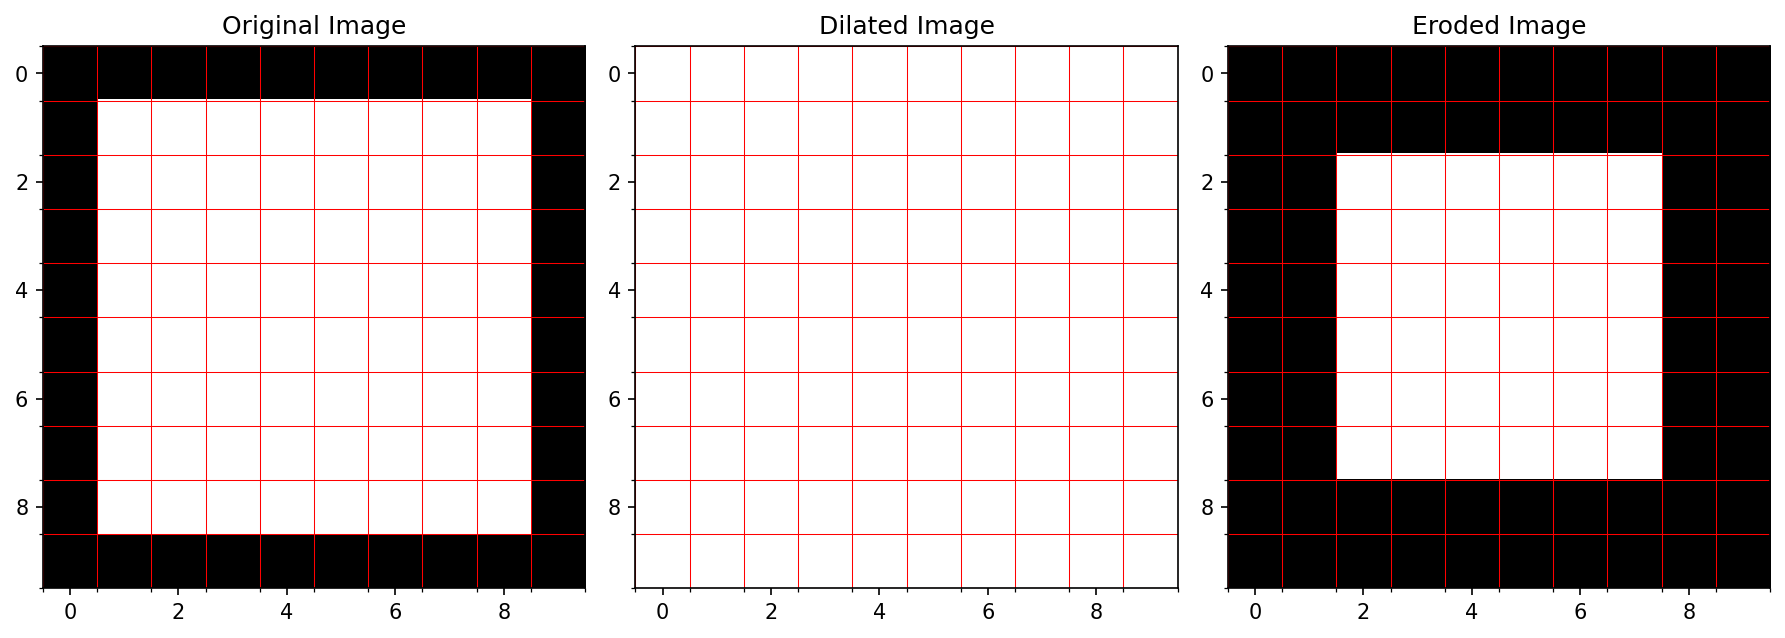
\includegraphics[width=\linewidth]{lab7.png}
    \caption{Morphological Basics. The central white shape is reduced via erosion and expanded via dilation (subject to padding constraints).}
    \label{fig:erodil}
\end{figure}

\subsection{Discussion}
The sliding window technique directly mirrors morphological theory. During erosion, if even a single zero from the background entered the $3 \times 3$ window, the minimum value became 0, effectively stripping the outermost layer of 1s from the square shape. Conversely, during dilation, the presence of a single 1 inside the window forced the center pixel to 1, causing the shape boundaries to expand outward.

\subsection{Conclusion}
The theoretical concepts of morphological erosion and dilation were verified through manual implementation. It was established that non-linear $\min$ and $\max$ filters combined with a structuring element effectively manipulate the boundaries of binary objects.

\pagebreak
% EXPERIMENT 8
\begin{center}
    \section{Experiment 8: Morphological Opening and Closing}
\end{center}

\subsection{Theory and Introduction}
Opening and closing are secondary morphological operations constructed by combining erosion and dilation in specific sequences \cite{gonzalez2018}.
\begin{itemize}
    \item \textbf{Opening ($A \circ B$):} Erosion followed by dilation. It smooths the contour of an object, breaks narrow isthmuses, and eliminates thin protrusions (noise).
    \item \textbf{Closing ($A \bullet B$):} Dilation followed by erosion. It smooths sections of contours, fuses narrow breaks and long thin gulfs, and fills small holes in the object.
\end{itemize}

\subsection{Methodology}
A binary image containing geometric artifacts (narrow bridges and gaps) was defined to test both operations using the previously developed erosion and dilation functions.

\subsubsection{Matrix Definition}
A customized binary matrix was structured to exhibit two large rectangular blocks connected by a narrow horizontal bridge, demonstrating vulnerabilities susceptible to opening and closing.

\subsubsection{Python Implementation}
The logic was executed sequentially. The \verb|manual_open()| function routed the output of \verb|manual_erode()| directly into \verb|manual_dilate()|. The \verb|manual_close()| function inverted this sequence.

\begin{multicols}{2}
    \inputminted{python3}{./assets/lab8.py}
\end{multicols}

\subsection{Results}
The geometric structures were fundamentally altered based on the operation sequence.

\begin{figure}[H]
    \centering
    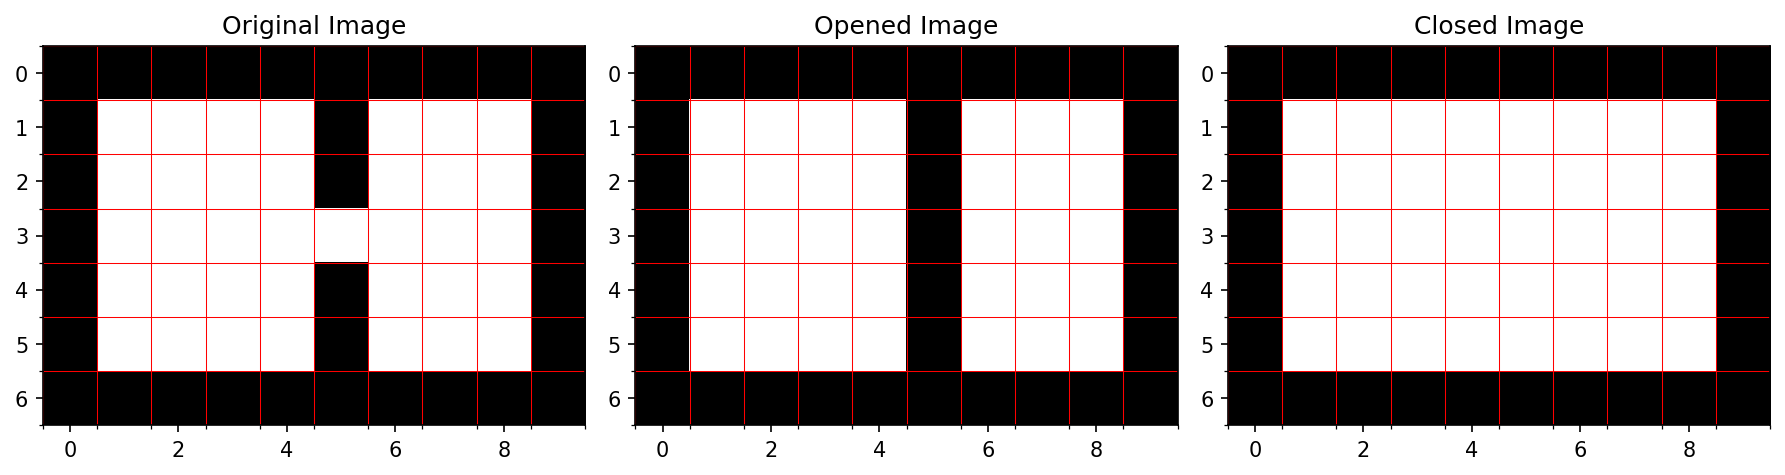
\includegraphics[width=\linewidth]{lab8.png}
    \caption{Opening and Closing. Left: Original shape with a bridge. Center: Opened image (bridge broken). Right: Closed image (bridge expanded and holes filled).}
    \label{fig:openclose}
\end{figure}

\subsection{Discussion}
The sequence of operations dictated the morphological outcome. In the Opening operation, the initial erosion completely obliterated the narrow bridge because the structuring element could not fit inside it. The subsequent dilation restored the primary blocks to their original size, but the bridge remained permanently erased. In the Closing operation, the initial dilation expanded the shapes, merging them across the gap. The subsequent erosion brought the outer boundaries back to normal, but the merged gap remained filled.

\subsection{Conclusion}
The utility of compound morphological operations was successfully demonstrated. It was verified that Opening is an effective tool for separating loosely connected objects and removing noise, while Closing is highly effective at fusing breaks and filling internal voids within objects.

\pagebreak
% EXPERIMENT 9
\begin{center}
    \section{Experiment 9: Hit-or-Miss Transform}
\end{center}

\subsection{Theory and Introduction}
The Hit-or-Miss Transform (HMT) is a basic morphological tool used for shape detection and pattern recognition within binary images. It utilizes a composite structuring element containing two parts: $B_1$ to detect the foreground shape (the "hit"), and $B_2$ to detect the local background (the "miss") \cite{gonzalez2018}.
$$
    A \circledast B = (A \ominus B_1) \cap (A^c \ominus B_2)
$$
A pixel is set to 1 in the output only if the foreground SE perfectly matches the image foreground, and the background SE perfectly matches the image background.

\subsection{Methodology}
A region of interest (ROI) was cropped from a larger image, and two specific structuring elements were configured to isolate a particular geometric pattern.

\subsubsection{Matrix Definition}
A region of interest was defined containing various noise elements and a few precise $2 \times 2$ square patterns. $SE_1$ was defined as a $2 \times 2$ matrix of 1s (to detect the square), while $SE_2$ was defined as the surrounding background elements (0s) necessary to ensure isolation.

\subsubsection{Python Implementation}
The SciPy \verb|binary_hit_or_miss| function (equivalent to MATLAB's \verb|bwhitmiss|) was utilized. The algorithm simultaneously applies erosion using $SE_1$ on the image and $SE_2$ on the complement of the image, returning the logical AND of the results.

\begin{multicols}{2}
    \inputminted{python3}{./assets/lab9.py}
\end{multicols}

\subsection{Results}
The transform successfully isolated the exact locations of the requested geometric patterns.

\begin{figure}[H]
    \centering
    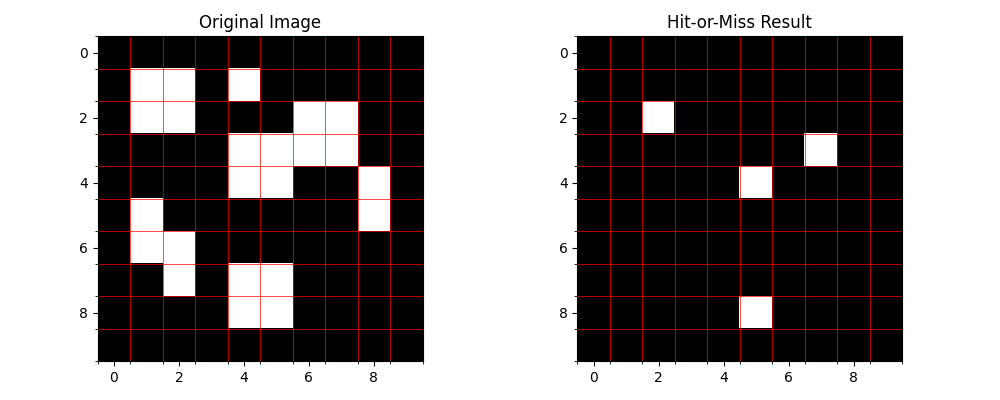
\includegraphics[width=\linewidth]{lab9.png}
    \caption{Hit-or-Miss Transform. Left: The original noisy matrix containing various shapes. Right: The single coordinates (hits) where the target $2 \times 2$ pattern was perfectly isolated.}
    \label{fig:hmt}
\end{figure}

\subsection{Discussion}
The stringent matching criteria of the HMT were clearly demonstrated. The transform ignored $2 \times 3$ rectangles and isolated 1s because they failed either the "hit" condition (foreground mismatch) or the "miss" condition (background mismatch). A positive result was only returned at the anchor point where the specific arrangement of 1s and surrounding 0s strictly matched the combined constraints of $SE_1$ and $SE_2$.

\subsection{Conclusion}
The Hit-or-Miss transform was validated as an extremely precise tool for structural analysis. It was shown that by carefully defining both the foreground and background structuring elements, specific patterns and features can be localized within complex binary images.


% REFERENCES

\pagebreak
\bibliographystyle{IEEEtran}
\renewcommand{\bibname}{References}
\addcontentsline{toc}{section}{References}
\bibliography{ref}

\end{document}